\documentclass[pscyr,titlepage]{hedreport}
\usepackage[utf8]{inputenc}
\usepackage[russian]{babel}
\usepackage{hedmaths}

\usepackage{graphicx}
\graphicspath{{images/}}

\usepackage{setspace}

\renewcommand{\thesection}{\arabic{section}.}
\renewcommand{\thesubsection}{\thesection\arabic{subsection}.}

\DeclareCaptionLabelFormat{figure}{Рисунок #2.}
\DeclareCaptionLabelFormat{table}{Таблица #2.}
\DeclareCaptionLabelSeparator{sep}{~}
\captionsetup{labelsep=sep,justification=centering,font=small}

\newcommand{\makemethodicpage}{
  \begin{titlepage}
    \singlespacing
    \newpage
    \begin{center}
      Министерство образования и науки Российской Федерации \\
      Федеральное государственное бюджетное образовательное \\
      учреждение высшего профессионального образования \\
      <<Волгоградский государственный технический университет>> \\
      Факультет электроники и вычислительной техники\\
      Кафедра физики
    \end{center}
    \vspace{9em}
    \begin{center}
      Лабораторная работа\\[.5em]
      \Large\scshape <<Исследование статических характеристик триода>>
    \end{center}
    \vspace{1em}    
    \begin{center}
      Методические указания
    \end{center}
    \vspace{3em}
    
    \vspace{\fill}
    \begin{center}
      Волгоград, \the\year
    \end{center}

  \end{titlepage}
}

\faculty{Факультет электроники и вычислительной техники}
\department{физики}
\type{Курсовая работа}
\subject{дисциплине\\<<Вакуумная и газоразрядная электроника>>}
\topic{Исследование статических характеристик триода}
\student[m]{студент группы Ф-469\\}
\teacher[m]{доцент Ковтун~Д.~Г.}

\begin{document}
  \maketitle
  \makemethodicpage
  \setcounter{page}{3}
  \section{Цель работы}

Ознакомиться с существующими исследовательскими ядерными реакторами и их
характеристиками, с помощью компьютерного моделирования рассчитать коэффициенты
размножения различных реакций и коэффициенты выгорания различных реакторов.

\section{Содержание работы}

\subsection{Основные понятия}

Ядерный (атомный) реактор -- устройство, в активной зоне которого
осуществляется контролируемая самоподдерживающаяся цепная реакция деления
ядер некоторых тяжелых элементов. Эта реакция представляет собой
самоподдерживающийся процесс деления ядер изотопов урана (или делящихся
изотопов других элементов) под действием элементарных частиц~-- нейтронов,
которые благодаря отсутствию электрического заряда легко проникают в атомные
ядра.

Основой работы ядерного реактора является самоподдерживающаяся цепная реакция
деления ядер урана, плутония и других трансурановых элементов.

Ядерные реакции -- это процесс перестройки ядра, сопровождающийся образованием
новых частиц и возникающий из-за взаимодействия с ядром элементарных частиц,
\( \gamma \)-квантов или других ядер. Общий вид ядерной реакции: \( a + A \to b + B \), где
\( a \), \( b \) -- соответственно налетающая и образующаяся частицы,
\( A \)~-- изначальное ядро (ядро-мишень), \( B \)~-- конечное ядро
(ядро-продукт).

Возможны и другие записи ядерных реакций: \( A(a, b)B \); \( (a, b) \).
Последняя используется, если речь идет об общем типе реакции, безотносительно к
частному виду мишени.

Совокупность бомбардирующих мишень частиц в определенном квантовом состоянии
называется входным каналом реакции.

Совокупность образовавшихся частиц в определенном квантовом состоянии
называется выходным каналом реакции.

Канал, по которому идет реакция, может быть различен при одинаковых входных каналах:
\begin{equation}
    \el{U}{235}{92} + \el{n}{1}{0} \to \el{La}{147}{57} + \el{Br}{87}{35} +
    2\el{n}{1}{0}; \quad
    \el{U}{235}{92} + \el{n}{1}{0} \to \el{Ba}{140}{56} + \el{Kr}{93}{36} +
    3\el{n}{1}{0}.
    \label{Udivide}
\end{equation}
И наоборот, канал реакции может быть одинаков при различных входных каналах.

Выход реакции -- это доля частиц пучка, испытавших взаимодействие с ядрами
мишени: \( W = \dfrac{\Delta N}{N} \), где \( N \) -- число налетающих частиц,
\( \Delta N \) -- число провзаимодействующих частиц. Выход можно связать с
так называемым полным эффективным сечением реакции: \( W = \sigma n \),
где \( n \) -- концентрация атомов мишени, \( \sigma \) -- полное эффективное
сечение реакции.

Эффективное сечение ядерной реакции \( \sigma' \) показывает вероятность
прохождения данной реакции за единицу времени при единичной плотности входного
канала. Полное эффективное сечение реакции \( \sigma \) представляет собой
сумму сечений реакций по всем каналам.

\subsection{Механизмы ядерных реакций}

Существует множество механизмов ядерных реакций. Рассмотрим механизмы
составного ядра и деления ядра.

Механизм составного (компаунд) ядра Бора: падающий на мишень нуклон в
результате столкновений передает энергию нуклонам в ядре, что приводит к
возникновению возбужденного ядра (компаунд-ядра). Через некоторое время
(значительно превосходящее ядерное время) в результате флуктуации один или
несколько нуклонов могут получить энергию, превышающую их энергию связи, и
покинуть ядро.

Общий вид реакции через компаунд-ядро: \( a + A \to C^* \to b + B \).

Механизм деления ядра рассматривается в рамках капельной модели. При поглощении
нейтрона ядро переходит в возбужденное состояние с интенсивными колебаниями.
Колеблясь, ядро принимает эллиптическую форму, проявляются положительно
заряженные центры. Если силы электростатического отталкивания превысят ядерные
силы, то ядро принимает гантелеобразную форму и, в итоге, делится (рис. \ref{picNDiv}).

Ядро \( \el{U}{238}{} \) делится только быстрыми нейтронами с \( E > 1 \)~МэВ.
Поэтому для поддержания ядерной реакции используют изотопы \(\el{U}{235}{}\).

\begin{figure}[h!]
    \centering
    \includegraphics[height=.35\textwidth]{nucdiv} \hspace*{6em}
    \includegraphics[height=.35\textwidth]{U235} \\
    \parbox{.35\textwidth}{\caption{Механизм деления ядра}\label{picNDiv}}
    \hspace*{2em}
    \parbox{.35\textwidth}{\caption{Спектр осколков деления урана-235}
    \label{picUDiv}}
\end{figure}

Реакции \eqref{Udivide} не единственные, которые могут происходить при делении
ядра урана-235. Спектр осколков деления (рис. \ref{picUDiv}) имеет два максимума: в области
атомных масс 90 и 140. Некоторые из осколков, имеющие большие сечения захвата
нейтронов, вредны для продолжения цепной реакции, иные, наоборот, являются
источниками дополнительных, запаздывающих, нейтронов.

При делении атома урана образуются сильно ионизированные осколки, являющиеся
радиоактивными и склонными к испусканию нейтронов. В среднем на каждый акт
деления происходит дополнительное появление 2,5 нейтронов. Это используется
для создания цепных реакций.

Минимальное условие возникновения цепной ядерной реакции определяется
коэффициентом размножения (воспроизводства) -- отношение числа тепловых
нейтронов (c \( E < 1 \)~МэВ) какого-либо одного поколения к числу тепловых
нейтронов предыдущего поколения:
\[
    K = \frac{n_i}{n_{i-1}}.
\]

Коэффициент размножения связан с мощностью реактора \( P \) степенным законом:
\begin{equation}
    P(t) = P_0 K^t,
    \label{eqPt}
\end{equation}
где \( P_0 \) -- техническая мощность реактора.

Система, в которой \( K = 1 \) называется критической (идеальный случай). В этом случае ядерные 
реакции происходят с постоянной скоростью, мощность реактора постоянна.

Система, в которой \( K > 1 \) называется надкритичной. В этом случае
интенсивность ядерных реакций нарастает, мощность реактора повышается. Долгая
работа в таком состоянии приводит к поломке реактора.

Система, в которой \( K < 1 \) называется подкритичной. В этом случае
интенсивность реакций спадает, следовательно, мощность реактора снижается.

\subsection{Ядерные реакторы}
Выделяют три большие группы ядерных реакторов:
\begin{enumerate}
    \item промышленные (энергетические), использующиеся в качестве источников
    тепловой энергии;
    \item исследовательские:
        \begin{itemize}
            \item использующиеся для получения различных видов излучения;
            \item размножители, наработчики новых радионуклидов, в том числе
            нового ядерного топлива или компонентов ядерного оружия
            (реакторы-конвертеры и реакторы-бридеры).
        \end{itemize}
\end{enumerate}

\begin{figure}[!ht]
    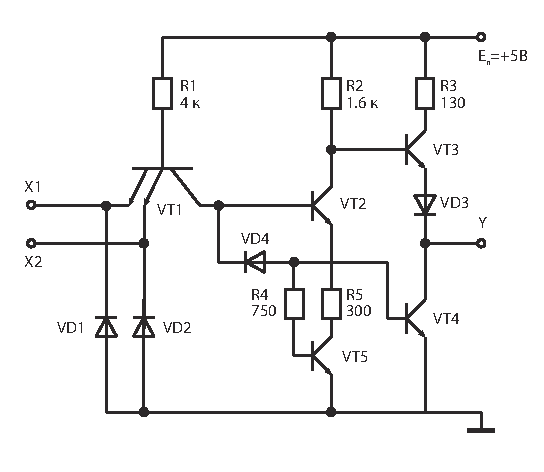
\includegraphics[width=.5\textwidth]{scheme} \hspace*{2em}
    \includegraphics[width=.35\textwidth]{active_zone} \\
    \parbox{.5\textwidth}{\caption{Принципиальная схема ядерного реактора}
    \label{picSch}} \hspace*{2em}
    \parbox{.35\textwidth}{\caption{Схема активной зоны ядерного реактора}
    \label{picAZ}}
\end{figure}

На рис. \ref{picSch} представлена общая схема строения ядерного реактора: 1 --
отражатель, 2 -- регулирующие стержни, 3 -- турбина, 4 -- генератор, 5 --
конденсатор, 6 -- парогенератор.

Схема активной зоны реактора -- места, где происходит процесс деления,~--
представлена на рис. \ref{picAZ}. Она содержит ядерное горючее 5, замедлитель 4, управляющий
стержень 1 и конструкционные материалы: радиационную защита 2, теплоизоляцию 3,
теплоноситель 6. Совокупность материалов, заполняющих активную зону
реактора называют мультиплицирующей (размножающей) средой.

Характеристика реактора, показывающая количество энергии, выделяющейся при
сгорании одной тонны топлива, называется коэффициентом выгорания \( k \), для
каждого реактора он является постоянной величиной. Коэффициент выгорания связан
со временем выгорания топлива \( t \):
\begin{equation}
    t = t_0 k_0 / k,
    \label{eqTk}
\end{equation}
где \( t_0 = 1000 \)~суток, \( k_0 = 1 \)~ГВт\( \cdot \)сут/т.

В данной работе представлены ядерные реакторы исследовательского типа.

Принципиально исследовательский реактор представляет генератор интенсивного
нейтронного потока, который является главным рабочим средством для исследования.

Исследовательский реактор должен обладать широким регулируемым спектром
физических характеристик нейтронного потока и обеспечивать возможность
проведения оригинальных научных экспериментов, зачастую в сложных и необычных
условиях.

От активной зоны реактора требуются высокие уровни удельной мощности, широкий
диапазон регулирования параметров, стабильность работы и полная гарантия
безопасности. Именно эти условия, прежде всего, должны обеспечиваться
свойствами и качественными характеристиками применяемого ядерного топлива. В
соответствии с целями и задачами ядерных исследований, выбор топлива базируется
на композиционных материалах с высокой концентрацией рабочего вещества.

В основном, такой реактор содержит водоохлаждаемую критическую активную зону,
собираемую по определенной схеме из тепловыделяющих элементов и их комбинаций,
называемых тепловыделяющими сборками (ТВС).

Активная зона исследовательского реактора представляет систему тепловыделяющих
сборок, составленных из коаксиального набора трубчатых тепловыделяющих
элементов, скрепленного дистанционирующими деталями и установочными
приспособлениями.

Каждый единичный тепловыделяющий элемент любой ТВС реакторов данного класса
представляет трубу круглого или многогранного сечения с трехслойной стенкой,
состоящей из среднего активного слоя и двух внешних покрытий, образующих
защитную оболочку.

При работе реактора в активном объеме тепловыделяющего элемента, содержащего
уран-235, развивается процесс ядерного деления с формированием потока нейтронов,
образованием осколочных элементов и выделением тепла. В данном случае и
накопление радиоактивных осколков, и тепловыделение представляют неизбежные
побочные явления, требующие локализации. Именно эту роль и выполняют защитные
оболочки, задерживающие осколочные элементы и отводящие тепловую энергию,
сохраняя активную зону от перегрева.

\section{Описание лабораторной установки}

Данная работа проводится расчетным методом на персональном компьютере. Для ее
выполнения используется специальная программа, которая загружена в компьютер.
Программа предназначена для ознакомления с существующими ядерными реакторами и
для расчета коэффициентов размножения и выгорания.

Функционально программа состоит из 2 основных блоков:
\begin{enumerate}
    \item блок выбора реактора;
    \item блок расчета коэффициентов.
\end{enumerate}

Для успешного выполнения работы надо иметь лишь элементарные навыки пользования
компьютером. В случае если таких навыков у студента нет, необходимо перед
выполнением работы проконсультироваться у преподавателя и выполнение работы
проводить только в присутствии лаборанта или преподавателя.

Перед выполнением работы договоритесь с преподавателем о количестве
производимых опытов.

\section{Порядок выполнения работы}

\begin{enumerate}
    \item Запустите программу.
    \item Выберите реактор, запишите мощность реактора.
    \item Переключитесь на вкладку ``Расчёт'', нажмите на кнопку ``Произвести
    расчёт''.
    \item Зарисуйте график зависимости мощности от времени и перепишите с
    графика зависимости количества оставшегося топлива от времени значение
    времени, при котором топливо закончится.
    \item Переключитесь на вкладку ``Реакторы'' и повторите пункты 2--4 для
    других реакторов необходимое число раз.
\end{enumerate}

\section{Обработка результатов}

\begin{enumerate}
    \item По формуле \eqref{eqPt} рассчитайте значение коэффициента размножения
    произошедшей реакции.
    \item По формуле \eqref{eqTk} рассчитайте значение коэффициента выгорания.
\end{enumerate}

К отчету лабораторной работы приложить графики зависимости \( P(t) \),
выполненные на миллиметровой бумаге, с подписанными значениями коэффициентов
размножения и выгорания.

\section{Контрольные вопросы}

\begin{enumerate}
    \singlespacing
    \itemsep -.5pt
    \item Дайте определение ядерной реакции.
    \item Какие механизмы ядерных реакций лежат в основе работы ядерных
    реакторов?
    \item Что называют коэффициентом размножения?
    \item Что такое ядерный реактор? Из каких основных частей он состоит?
    \item Опишите схему активной зоны ядерного реактора.
\end{enumerate}

\section{Список рекомендуемой литературы}
\begin{enumerate}
    \item Ракобольская И. В. Ядерная физика. М.: Изд. Моск. университета,
    1971.~-- 296 с.
    \item Фейнсберг С. М., Шихов С. Б., Троинский В. Б. Теория ядерных
    реакторов. Т. 1. Элементарная теория реакторов: Учебник для вузов -- М.:
    Атомиздат, 1978. -- 400 с.
    \item Бекман И. Н. Ядерная индустрия: курс лекций. Лекция 12: Ядерные
    реакторы.
    \item Игнатьев П. П. Энергия -- это сама жизнь.
\end{enumerate}
  
  \newpage
  \section*{Паспортные характеристики}
  \begin{table}[ht]
    \center
    \caption*{Семейство анодно-сеточных характеристик}
    \begin{tabular}{|m{.15\textwidth}|C{.1}|*{7}{C{.07}|}} \hline
      \multirow{5}{*}{\( U_{a_{01}} = \)~В} &
        \( U_c \),~В &&&&&&& \\ \cline{2-9}
      & \( I_{a_1} \),~мА &&&&&&& \\ \cline{2-9}
      & \( I_{a_2} \),~мА &&&&&&& \\ \cline{2-9}
      & \( I_{a_3} \),~мА &&&&&&& \\ \cline{2-9}
      & \( \average{I_a} \),~мА &&&&&&& \\ \hline
      \multirow{5}{*}{\( U_{a_{02}} = \)~В} &
        \( U_c \),~В &&&&&&& \\ \cline{2-9}
      & \( I_{a_1} \),~мА &&&&&&& \\ \cline{2-9}
      & \( I_{a_2} \),~мА &&&&&&& \\ \cline{2-9}
      & \( I_{a_3} \),~мА &&&&&&& \\ \cline{2-9}
      & \( \average{I_a} \),~мА &&&&&&& \\ \hline
      \multirow{5}{*}{\( U_{a_{03}} = \)~В} &
        \( U_c \),~В &&&&&&& \\ \cline{2-9}
      & \( I_{a_1} \),~мА &&&&&&& \\ \cline{2-9}
      & \( I_{a_2} \),~мА &&&&&&& \\ \cline{2-9}
      & \( I_{a_3} \),~мА &&&&&&& \\ \cline{2-9}
      & \( \average{I_a} \),~мА &&&&&&& \\ \hline
      \multirow{5}{*}{\( U_{a_{04}} = \)~В} &
        \( U_c \),~В &&&&&&& \\ \cline{2-9}
      & \( I_{a_1} \),~мА &&&&&&& \\ \cline{2-9}
      & \( I_{a_2} \),~мА &&&&&&& \\ \cline{2-9}
      & \( I_{a_3} \),~мА &&&&&&& \\ \cline{2-9}
      & \( \average{I_a} \),~мА &&&&&&& \\ \hline
      \multirow{5}{*}{\( U_{a_{05}} = \)~В} &
        \( U_c \),~В &&&&&&& \\ \cline{2-9}
      & \( I_{a_1} \),~мА &&&&&&& \\ \cline{2-9}
      & \( I_{a_2} \),~мА &&&&&&& \\ \cline{2-9}
      & \( I_{a_3} \),~мА &&&&&&& \\ \cline{2-9}
      & \( \average{I_a} \),~мА &&&&&&& \\ \hline
    \end{tabular}
  \end{table}
  
  \pagebreak
  
  \begin{table}[ht]
    \center
    \caption*{Семейство анодно-сеточных характеристик}
    \begin{tabular}{|m{.15\textwidth}|C{.1}|*{7}{C{.07}|}} \hline
      \multirow{5}{*}{\( U_{c_{01}} = \)~В} &
        \( U_a \),~В &&&&&&& \\ \cline{2-9}
      & \( I_{a_1} \),~мА &&&&&&& \\ \cline{2-9}
      & \( I_{a_2} \),~мА &&&&&&& \\ \cline{2-9}
      & \( I_{a_3} \),~мА &&&&&&& \\ \cline{2-9}
      & \( \average{I_a} \),~мА &&&&&&& \\ \hline
      \multirow{5}{*}{\( U_{c_{02}} = \)~В} &
        \( U_a \),~В &&&&&&& \\ \cline{2-9}
      & \( I_{a_1} \),~мА &&&&&&& \\ \cline{2-9}
      & \( I_{a_2} \),~мА &&&&&&& \\ \cline{2-9}
      & \( I_{a_3} \),~мА &&&&&&& \\ \cline{2-9}
      & \( \average{I_a} \),~мА &&&&&&& \\ \hline
      \multirow{5}{*}{\( U_{c_{03}} = \)~В} &
        \( U_a \),~В &&&&&&& \\ \cline{2-9}
      & \( I_{a_1} \),~мА &&&&&&& \\ \cline{2-9}
      & \( I_{a_2} \),~мА &&&&&&& \\ \cline{2-9}
      & \( I_{a_3} \),~мА &&&&&&& \\ \cline{2-9}
      & \( \average{I_a} \),~мА &&&&&&& \\ \hline
      \multirow{5}{*}{\( U_{c_{04}} = \)~В} &
        \( U_a \),~В &&&&&&& \\ \cline{2-9}
      & \( I_{a_1} \),~мА &&&&&&& \\ \cline{2-9}
      & \( I_{a_2} \),~мА &&&&&&& \\ \cline{2-9}
      & \( I_{a_3} \),~мА &&&&&&& \\ \cline{2-9}
      & \( \average{I_a} \),~мА &&&&&&& \\ \hline
      \multirow{5}{*}{\( U_{c_{05}} = \)~В} &
        \( U_a \),~В &&&&&&& \\ \cline{2-9}
      & \( I_{a_1} \),~мА &&&&&&& \\ \cline{2-9}
      & \( I_{a_2} \),~мА &&&&&&& \\ \cline{2-9}
      & \( I_{a_3} \),~мА &&&&&&& \\ \cline{2-9}
      & \( \average{I_a} \),~мА &&&&&&& \\ \hline
    \end{tabular}
  \end{table}
  
\end{document}
